%%%%%%%%%%%%%%%%%%%%%%%%%%%%%%%%%%%%%%%%%%%%%%%%%%%%%%%%%%%%%%%%%%%%%%%%%%%%%%%%
%2345678901234567890123456789012345678901234567890123456789012345678901234567890
%        1         2         3         4         5         6         7         8

\documentclass[letterpaper, 12 pt, conference]{ieeeconf}  % Comment this line out
                                                          % if you need a4paper
%\documentclass[a4paper, 10pt, conference]{ieeeconf}      % Use this line for a4
                                                          % paper

\IEEEoverridecommandlockouts                              % This command is only
                                                          % needed if you want to
                                                          % use the \thanks command
\overrideIEEEmargins
% See the \addtolength command later in the file to balance the column lengths
% on the last page of the document

\usepackage[utf8]{inputenc}
\usepackage[T1]{fontenc}
\usepackage{graphicx}


% The following packages can be found on http:\\www.ctan.org
%\usepackage{graphics} % for pdf, bitmapped graphics files
%\usepackage{epsfig} % for postscript graphics files
%\usepackage{mathptmx} % assumes new font selection scheme installed
%\usepackage{mathptmx} % assumes new font selection scheme installed
%\usepackage{amsmath} % assumes amsmath package installed
%\usepackage{amssymb}  % assumes amsmath package installed

\title{\LARGE \bf
CENG 435 DATA COMMUNICATION AND NETWORKING \\ TERM PROJECT-1 GROUP 75
}

%\author{ \parbox{3 in}{\centering Huibert Kwakernaak*
%         \thanks{*Use the $\backslash$thanks command to put information here}\\
%         Faculty of Electrical Engineering, Mathematics and Computer Science\\
%         University of Twente\\
%         7500 AE Enschede, The Netherlands\\
%         {\tt\small h.kwakernaak@autsubmit.com}}
%         \hspace*{ 0.5 in}
%         \parbox{3 in}{ \centering Pradeep Misra**
%         \thanks{**The footnote marks may be inserted manually}\\
%        Department of Electrical Engineering \\
%         Wright State University\\
%         Dayton, OH 45435, USA\\
%         {\tt\small pmisra@cs.wright.edu}}
%}

\author{Orhan ALBAYRAK$^{1}$ and Mustafa GÖNEN$^{2}$% <-this % stops a space
\thanks{*This report was prepared any Orhan and Mustafa}% <-this % stops a space
\thanks{$^{1}$Orhan is with Department of Computer Engineering, METU - ANKARA e2264471
        {\tt\small}}%
\thanks{$^{2}$Mustafa is with the Department of Computer Engineering, METU - ANKARA e2264547
        {\tt\small www.mustafa.gonenn.com}}%
}


\begin{document}



\maketitle
\thispagestyle{empty}
\pagestyle{empty}


%%%%%%%%%%%%%%%%%%%%%%%%%%%%%%%%%%%%%%%%%%%%%%%%%%%%%%%%%%%%%%%%%%%%%%%%%%%%%%%%
\begin{abstract}

This document is a report was prepared for Data Communications and Networking Term Project in 2019. 

\end{abstract}


%%%%%%%%%%%%%%%%%%%%%%%%%%%%%%%%%%%%%%%%%%%%%%%%%%%%%%%%%%%%%%%%%%%%%%%%%%%%%%%%
\section{DESIGN PART}

\subsection{ Project Overview }

In this project our main purpose is to design and implement the nodes of a network that the components are Source, Router-1, Router-2, Router-3 and Destination. We imported our codes to all nodes with using UDP Protocol. In our scenario each node have a client/server application at the same time, to be able to receive packets, send acks, send packets and receive acks. Besides, source just sends packet and receives acks, destination just receives packet and sends acks. They are tested that the links are bound and communicated each other. RTT values are measured by R1, R2, R3 for each hop(node). After that link costs are measured, and that information reserved in routers as a TXT file. Routing logic for the nodes are processing in Application Level. After forward and storing the costs for all link the shortest path is determined from source node ”s” to the destination node ”d” based on Dijkstra Algorithm. Thanks to this experiment know-ledges, we chose one short path regarding as Dijkstra algorithm and end-to-end delays are measured with three experiments.

\subsection{ Design Approach }
The first rule is that, we have to the apply our scripts for each node including both client and server UDP applications. Then, we designed a scenario for this issue that measuring the link costs, calculating end-to-end delay and do some experiments with delays. As a first, we will briefly call source,router1,router2,router3 and destination as source, r1, r2, r3 and dest respectively. Because we need to have end-to-end delay in dest node and calculate link costs, we embedded time info to these packets beside message. In our scenario, source's role is to send byte streams to r1, r2 and r3 nodes and receiving responses of packets with using UDP Protocols. Then, r1's role is that, beside sending acks to source, it also sends packets to r2 and dest with receiving acks as well as receiving packets from source and sending the responses of packets to source. R2's role is receiving packets from source r1 and r2 and then sending messages to source finally receive responses of messages. R3's role is that, beside sending acks to source, it also sends packets to r2 and dest with receiving acks as well as receiving packets from source and sending the responses of packets to source. In destination node,first receiving all packets transferred from routers and calculation for end-to-end delay for whole process. Then, stored time info (costs for each link, end-to-end delay and delays for exp. ) in a TXT file.  In this design, all nodes can behave as a server and client with using UDP Protocol following assignment specifications.

\section{IMPLEMENTATION PART}

\subsection{Steps We Follow}

We want to explain our steps that we followed during implementation process. We started by using Python language to write our scripts for each node separately. Because Python language is more useful and effective in socket programming. Then we created our slices in our project on GENI Platform. In order to have some information about GENI, we used given tutorials and some document on the Internet. After gripping GENI, we tried to understand our Topology with all details. Afterwards, we imported our topology XML file on to GENI Platform. Finally, we could access all details of our project like IP address, interface information and port numbers belongs to source routers and destination.     

\subsection{About Geni Platform}
Since we are not familiar to GENI Platform, we followed lab0 document before takink our GENI accounts. After some experience on GENI, we could easily take account, create slices and control virtual machines using SSH connections.

\subsection{Implementation Process}
Before start our implementation, we discovered client and server applications in Python Socket Programming, creating socket function, closing socket function, sending a random message from client to server and receiving response from server. After we understand this concepts, we designed a client/server application between source node and router-1. We developed two script 's.py' for source node 'r1.py' for router-1 for this application. In this our first attempt, source were going to behave as a client and send a random message to router-1 while router-1 were behaving as a server. To do this, we imported socket and sys libraries then we create a client UDP socket, we configured server IP address and port number and we created just a random message in our 's.py' script. In 'r1.py' script , we tried to receive this random message and then, send responses of this random message to source. So in 'r1.py' script acting as a server, we created a server UDP client socket. We configured IP addresses and port numbers again and bind socket to the port. Then we could do receiving message from source and sending ack of message to client. In this manner, we could basically do first link between 'source-r1' with two script 's.py' and 'r1.py'. After this first part; we were going to aim sends and receives multiple messages on this link 'source-r1'. We increased the number of packet to '1000 packets'. Then, we decided to embed time to measure link cost. At the end of this process, we send '1000 packet' from source to r1 with embedded time info then, we could estimate link cost averaging calculated RTT value for one packet over 1000 packet. Afterward, we applied this approach to 'soruce-r1', 'source-r2', 'r1-r2', 'r3,r1', 'r1-dest', 'r2-dest', 'r3-dest', and 'r3-r1' as we done yet in 'source-r1'.  After we have completed to all discrete link, we had to plan our scenario for all nodes (source, r1, r2, r3, and dest). While we designing our own approach, we have considered that each hope have to send and receive message at the same time, so it is able to be make multiple request from other nodes. In our scenario, source will send packets to Router-1 Router-2 and Router-3 at the same time while routers are listening to source. Then, routers send their acks packets to source. Then, r1 send packets and receiving acks to r2 and dest at the same time. R3 send packets and receiving acks to r2 and dest with making multiple requests at the same time. Dest is listening routers and send their acks with making multiple requests again. To be able to catch up this flow chart between nodes, we run our scripst d, r2, r1, r3 and source respectively. After running all scripts and completing all request simultaneously, we get link costs for all hops. We have shown all costs in Figure-1.


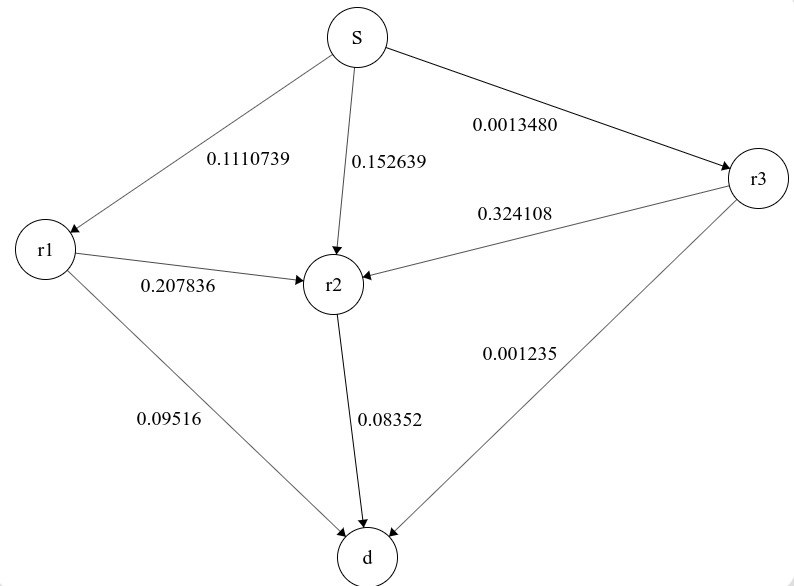
\includegraphics[width=8.5cm, height=7cm]{link-cost.jpeg}

\begin{center}
Figure-1
\end{center}

These cost are belongs links that connecting nodes. We used these RTT values to find the shortest path from source to destination. Now, we have shown routing tables to understand shortest path from source to destination.\\

\subsection{ Avaible Paths }

\begin{center}
Routing I
\end{center}

\begin{center}
 \begin{tabular}{||c c||} 
 \hline
 Destination & Send to  \\ [0.25ex] 
 \hline\hline
 S & R1  \\ 
 \hline
 R1 & R2  \\
 \hline
 R2 & D \\
 
 \hline
\end{tabular}
\end{center}




\begin{center}
Routing II
\end{center}

\begin{center}
 \begin{tabular}{||c c||} 
 \hline
 Destination & Send to  \\ [0.25ex] 
 \hline\hline
 S & R3  \\ 
 \hline
 R3 & R2  \\
 \hline
 R2 & D \\
 
 \hline
\end{tabular}
\end{center}

\begin{center}
Routing III
\end{center}

\begin{center}
 \begin{tabular}{||c c||} 
 \hline
 Destination & Send to  \\ [0.25ex] 
 \hline\hline
 S & R2  \\ 
 \hline
 R2 & D  \\
 
 \hline
\end{tabular}
\end{center}

\begin{center}
Routing IV
\end{center}

\begin{center}
 \begin{tabular}{||c c||} 
 \hline
 Destination & Send to  \\ [0.25ex] 
 \hline\hline
 S & R1  \\ 
 \hline
 R1 & D  \\
 
 \hline
\end{tabular}
\end{center}

\begin{center}
Routing V
\end{center}

\begin{center}
 \begin{tabular}{||c c||} 
 \hline
 Destination & Send to  \\ [0.25ex] 
 \hline\hline
 S & R3  \\ 
 \hline
 R3 & D  \\
 
 \hline
\end{tabular}
\end{center}

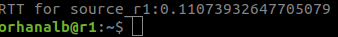
\includegraphics[width=8cm, height=2cm]{s-r1.png}

\begin{center}
s-r1
\end{center}



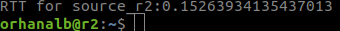
\includegraphics[width=8cm, height=2cm]{s-r2.png}

\begin{center}
s-r2
\end{center}



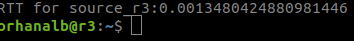
\includegraphics[width=8cm, height=2cm]{s-r3.png}

\begin{center}
s-r3
\end{center}



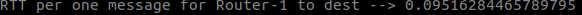
\includegraphics[width=8cm, height=1cm]{r1-d.png}

\begin{center}
r1-d
\end{center}



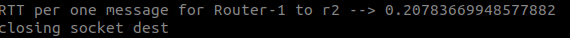
\includegraphics[width=8cm, height=2cm]{r1-r2.png}

\begin{center}
r1-r2
\end{center}


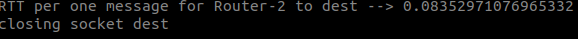
\includegraphics[width=8cm, height=2cm]{r2-d.png}

\begin{center}
r2-d
\end{center}



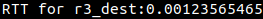
\includegraphics[width=8cm, height=1cm]{r3-dest.png}

\begin{center}
r3-d
\end{center}

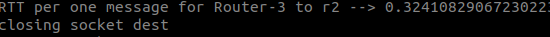
\includegraphics[width=8cm, height=1cm]{r3-r2.png}

\begin{center}
r3-r2
\end{center}

\section{Experimental Results}


We firstly use some tools to sync nodes and add delays with different delays.
The first command is -->
   sudo  ntpdate -u pool.ntp.org
then-->
for each part of the experiment we used the commands below:
### Shows current delay
   tc qdisc show dev [interface name]  
### Adds delay to node
   tc qdisc add dev [interface name] root netem delay 20ms 5ms distribution normal
### Removes the current delay
   tc qdisc del dev [interface name] root
Experiment results
In this part we create the experiment script files for s, r3, d. We choose this route from the previous part because the less link cost (we find this result from Dijkstra algorithm). We send messages from s to r3 then r3 is waiting to send the message to s when d sends the message to r3 then r3 sends to message back to s. We make the time measurement at s node. When s node starts sending message we take time measurement. After message comes from r3 we  take another time measurement. By finding the difference between these two we calculate the end-to-end delay.\\
We applied 4 experiment on nodes :\\
At first we measured end-to-end delay without emulation delay and we got the result :\\ 1.98513 ms\\
Then we add 20 ms delay to all links and we got the result:\\
73.56345 ms\\
After that we add 40 ms delay to all links and we got the result:\\
142.3544 ms\\
Finally we add 50 ms delay to all links and we got the result:\\
180.32435 ms\\


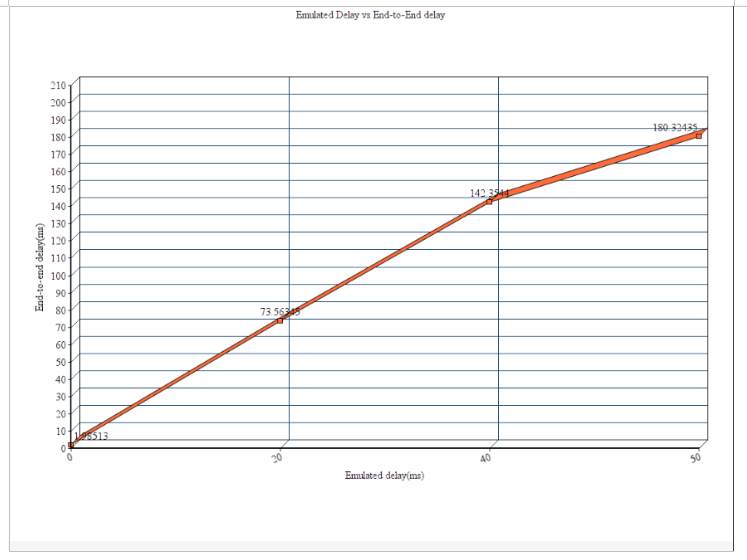
\includegraphics[width=9cm, height=8cm]{graph.png}

\begin{center}
Figure: End-to-end Delay vs Emulated Delay Graph
\end{center}

\section{NETEM COMMANDS}

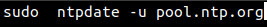
\includegraphics[width=9cm, height=2cm]{1.png}

\begin{center}
Command I
\end{center}

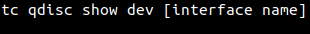
\includegraphics[width=9cm, height=2cm]{2.png}

\begin{center}
Command II
\end{center}

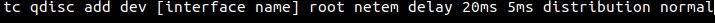
\includegraphics[width=9cm, height=2cm]{3.png}

\begin{center}
Command III
\end{center}

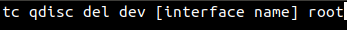
\includegraphics[width=9cm, height=2cm]{son.png}

\begin{center}
Command IV
\end{center}




\end{document}
